\documentclass{beamer}

\usepackage[utf8]{inputenc}
\usepackage[english]{babel}
\usepackage[T1]{fontenc}

\usepackage{kpfonts}
\usepackage{helvet}

\usepackage{booktabs}
\usepackage{icomma}
\usepackage{listings}
\usepackage{color}

\usepackage{siunitx}

\usepackage{algpseudocode}

%\usepackage{mhchem}

\definecolor{matcom}{rgb}{0.0,0.5,0.0} 
\definecolor{matkey}{rgb}{0.0,0.0,1.0} 
\definecolor{matstr}{rgb}{0.0,0.5,0.0} 
\definecolor{matbg}{rgb}{0.9,0.9,0.9}

\lstset{
numbers=left,
numberstyle=\tiny\color{gray},
language=Matlab,
basicstyle=\ttfamily,
extendedchars=true,
inputencoding=latin1,
showstringspaces=false,
numberstyle=\ttfamily,
keywordstyle=\color{matkey},
stringstyle=\color{matstr},
commentstyle=\color{matcom},
backgroundcolor=\color{matbg},
frame=lines,
breaklines=true
}

\newcommand{\dimuon}{\mu^+ \mu^-}

\usetheme{Copenhagen}
\usecolortheme{spruce}
\usefonttheme{structureitalicserif}

\setbeamertemplate{items}[circle]
\mode<presentation>

\title[Thundersone urval]{GUI för kontrollerat slumpurval av kort för brädspelet Thunderstone}
\author[P. Engström, A. Remmers]{Per Engström \& Alexis Remmers \\[0.5cm] 
\normalsize \emph{Projekt} \\
\normalsize \emph{Introduktion till informationsteknologi, 10hp}}

\begin{document}

\begin{frame}[plain]
	\centering
	\titlepage
\end{frame}

\begin{frame}
\frametitle{Bakgrund}
\framesubtitle{Thunderstone}

\begin{columns}%[T]
    \begin{column}{.5\textwidth}
        \centering
        
\includegraphics[width=\textwidth]{thunderstone-3dbox.png}
    \end{column}
    \begin{column}{.5\textwidth}
        \begin{itemize}
            \item Kortspel med slumpat urval
            \pause
            \item Till varje spel slumpas:
            \begin{itemize}
                \item 3 (av 8) 'Monster'-kort
                \item 4 (av 11) 'Hero'-kort
                \item 8 (av 19) 'Village'-kort
            \end{itemize}
        \end{itemize}
    \end{column}
\end{columns}

\end{frame}

\begin{frame}
    \frametitle{Bakgrund}
    \framesubtitle{Krav på urvalet}
    
    \begin{columns}%[T]
        \begin{column}{.5\textwidth}
            \centering
            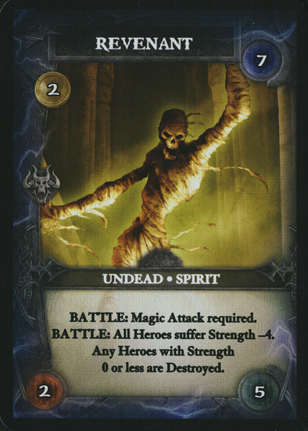
\includegraphics[width=\textwidth]{Rvnant.png}
        \end{column}
        \begin{column}{.5\textwidth}
            \begin{itemize}
                \item Alla kombinationer är inte lika balanserade
                \pause
                \item Korten definierar 'krav'
                \item Kan vi inte bara slumpa fram urval som uppfyller alla dessa krav?
            \end{itemize}
        \end{column}
    \end{columns}
\end{frame}

\begin{frame}
    \frametitle{Demonstation}
    
    \begin{quote}
        Buy my mixtape
    \end{quote}
\end{frame}

\begin{frame}
    \frametitle{Söndra och härska}
    \framesubtitle{Red Alert}
    
   
    
    \begin{columns}
        \begin{column}{0.5\textwidth}
             \begin{itemize}
                 \item Motor (ca 40 funktioner)
                 \begin{itemize}
                     \item Lagring av kort
                     \item Skapa urvalspreferenser
                     \item Korrekt urval givet preferenser
                     \begin{itemize}
                         \item Kontrollera krav
                        \end{itemize}
                        \item Implementering av \textsc{gui}
                    \end{itemize}
                    \item Grafik
                    \begin{itemize}
                        \item GTK
                        \item Glade
                    \end{itemize}
                \end{itemize}
        \end{column}
        \begin{column}{0.5\textwidth}
            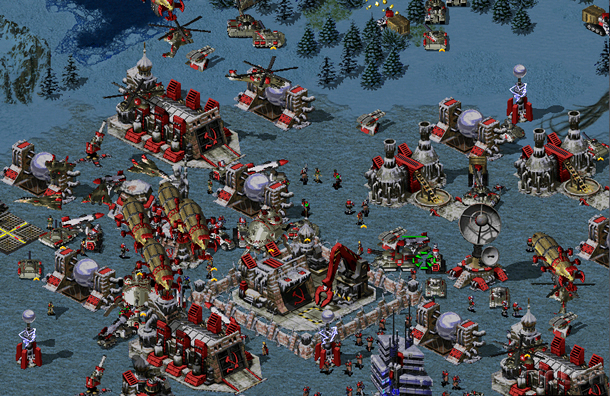
\includegraphics[width=\textwidth]{ra2.jpg}
        \end{column}
    \end{columns}

\end{frame}

\begin{frame}
    \frametitle{Datastrukturer}
    \begin{columns}
    \begin{column}{0.5\textwidth}
        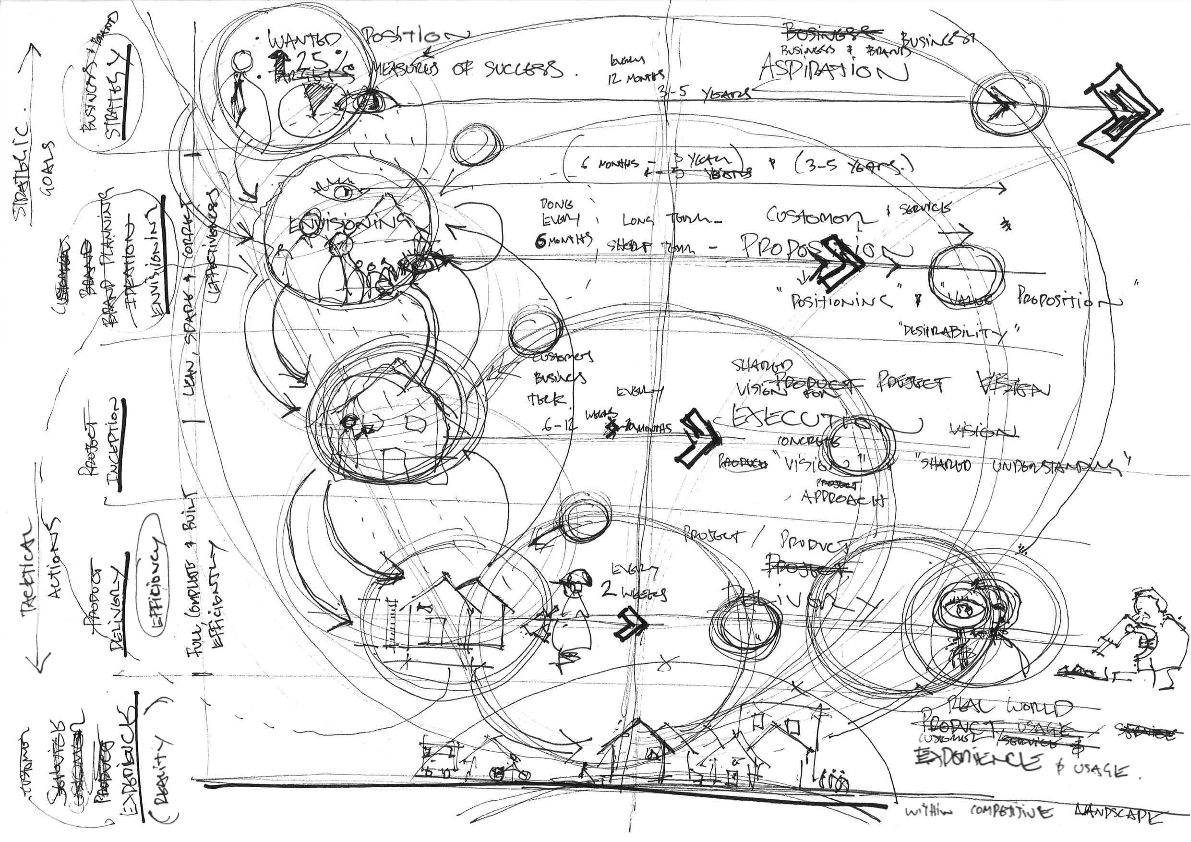
\includegraphics[width=\textwidth]{mess.png}
    \end{column}
    \begin{column}{0.5\textwidth}
        \begin{itemize}
            \item Tuplar
            \begin{itemize}
                \item Kort
            \end{itemize}
            \item Mängder
            \begin{itemize}
                \item Ett antal kort
            \end{itemize}
            \item Listor
            \begin{itemize}
                \item Grafiska kortlistor
            \end{itemize}
            \item Klasser
            \begin{itemize}
                \item Ett urval
                \item Urvalspreferenser
            \end{itemize}
            \item XML
            \begin{itemize}
                \item Layout
            \end{itemize}
        \end{itemize}
    \end{column}
    \end{columns}
    
    
    
\end{frame}

\begin{frame}
    \frametitle{Algoritmer}
    \framesubtitle{Korrekt urval}
    
    \begin{columns}
        \begin{column}{0.5\textwidth}
            
\includegraphics[width=\textwidth]{inf.jpg}
        \end{column}
        \begin{column}{0.5\textwidth}
            getSelection()
            \begin{enumerate}
                \item \textbf{while} True
                \begin{enumerate}
                    \item selection = randomSelection()
                    \item \textbf{if} selection.validate()
                    \begin{enumerate}
                        \item \textbf{break}
                    \end{enumerate}
                \end{enumerate}
                \item \textbf{return} selection
            \end{enumerate}
        \end{column}
    \end{columns}

    
  
\end{frame}

\begin{frame}
    \frametitle{Algoritmer}
    \framesubtitle{Kravkontroll}
    
    Validate()
    \begin{enumerate}
        \item \textbf{for} card \textbf{in} allCards
        \begin{enumerate}
            \item \textbf{for} dependencies \textbf{in} card
            \begin{enumerate}
                \item \textbf{if} \textbf{not} depChk(dependency, AllCards) \textbf{return} False
            \end{enumerate}
        \end{enumerate}
        \item \textbf{return} True
    \end{enumerate}
    
    \vfill
    
    depChk(dependency, allCards)
    \begin{enumerate}
        \item \textbf{for} card \textbf{in} allCards
        \begin{enumerate}
            \item \textbf{if} card \emph{provides} dependency \textbf{return} True
        \end{enumerate}
        \item \textbf{return} False
    \end{enumerate}
\end{frame}

\begin{frame}
    \frametitle{Funktioner och kontrollstrukturer}
    
    
\end{frame}

\begin{frame}
    \frametitle{Reflektion}
    
    \begin{itemize}
        \item Programbibliotek finns i många (och inte nödvändigtvis kompatibla) versioner
        \begin{itemize}
            \item Två stora versioner: \textbf{GTK 2.x} och GTK 3.x
            \item Glade 3.18 för GTK 3 och \textbf{Glade 3.8} för GTK 2
            \item \textbf{PyGTK} för GTK 2 i python, GOBject för GTK 3
        \end{itemize}
        \pause
        \item GTK är ett moget och inte helt svåranvänt gränsnittsramverk
        \pause
        \item Glade är guds gåva till nybörjaren
        \pause
        \item Klasser kan användas till mer än man tror, inte bara för lagring
        \pause
        \item Git (och GitHub) fungerar utmärkt när man samarbetar med kod
        \pause
        \item Man kan lätt dela upp koden i filer för att organisera sin kod
    \end{itemize}
\end{frame}

\begin{frame}
    \frametitle{Frågor}
    \framesubtitle{Frågor}
    
\includegraphics[width=\textwidth]{xkcd.jpg}
\end{frame}

\end{document}